
\onecolumn
\begin{inctext}[paper=graphics]
  \begin{tikzpicture}
    \coordinate (below left) at (0in,0in);
    \coordinate (above right) at (8.5in,11in);
    \path[use as bounding box] (below left) rectangle (above right);
    \draw[very thin, Seashell2] (below left) grid (above right);
    \draw (0,25) node[right]
      {\fontsize{100pt}{0pt}\selectfont
        \textbf{Math\textit{\textcolor{DodgerBlue2}{P}}robs}};
    \foreach \pos/\char in {21/数,17.5/学,14/题,10.5/集} {
      \draw (0,\pos) node[right]
        {\fontsize{100pt}{0pt}\selectfont \textbf{\textit{\char}}}; }
    \fill[DeepSkyBlue2] (17.5,23.9) rectangle (22,25.5);
    \fill[DarkSlateGray3] (10,0) -| (22,8) -- cycle;
    \draw (21.5,3) node[left]
      {\fontsize{60pt}{0pt}\selectfont
      \textcolor{DarkSlateGray1}{\textbf{\texttt{0000}}}};
    \draw (21.5,1) node[left]
      {\fontsize{60pt}{0pt}\selectfont
      \textcolor{DarkSlateGray1}{\textbf{-- \texttt{003F}}}};
    \draw (17.5,24.7) node[right] {
      \begin{minipage}{10cm}
        \fontsize{10pt}{10pt}\selectfont \textcolor{Azure1}
        {Copyright \copyright\ 2024 \\
          \textbf{Liu One} \\ \emph{All rights reserved.}}
      \end{minipage} };
    \draw (0,6.9) node[right] {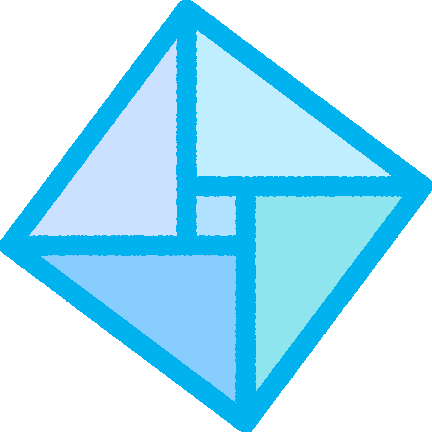
\includegraphics[scale=.45]{covers/logo}};
    \draw (2,4) node {\Huge\textcolor{RoyalBlue1}{\textbf{VOL.}}};
    \draw (2,2) node
      {\fontsize{100pt}{0pt}\selectfont\textcolor{RoyalBlue2}{\textbf{1}}};
    \draw (10,8) node {
      \begin{minipage}{3cm}
        \footnotesize \textit{
        \raggedright Heron公式 \\
        $S^2 = p(p - a)(p - b)(p - c),$ \\
        $p = \sfrac{a + b + c}2$ \\
        \raggedleft ——简洁的对称美 \\ }
      \end{minipage} };
    \begin{scope}[shift={(5.5,16)}, scale=1.7, very thick]
      \def\Ax{0} \def\Ay{0} \def\Bx{7} \def\By{0} \def\Cx{5} \def\Cy{4}
      \coordinate[label=above left:$A$] (A) at (\Ax,\Ay);
      \coordinate[label=above right:$B$] (B) at (\Bx,\By);
      \coordinate[label=above:$C$] (C) at (\Cx,\Cy);
      \coordinate (Dbisector) at
        ({\calcbisectorx\Bx\By\Ax\Ay\Cx\Cy},
        {\calcbisectory\Bx\By\Ax\Ay\Cx\Cy});
      \coordinate (Ebisector) at
        ({\calcbisectorx\Ax\Ay\Bx\By\Cx\Cy},
        {\calcbisectory\Ax\Ay\Bx\By\Cx\Cy});
      \path[name path=OA] (A) -- (Dbisector);
      \path[name path=OB] (B) -- (Ebisector);
      \path[name intersections={of=OA and OB}]
        coordinate[label=above right:$O$] (O) at (intersection-1);
      \coordinate[label=right:$D$] (D) at ($ (B)!(O)!(C) $);
      \coordinate[label=above:$E$] (E) at ($ (A)!(O)!(C) $);
      \coordinate[label=below:$F$] (F) at ($ (A)!(O)!(B) $);
      \coordinate[label=right:$M$] (M) at ({(7+sqrt(41))/2+sqrt(5)},0);
      \path[name path=BN] (B) -- ($ (B)!1! 90:(A) $);
      \path[name path=ON] (O) -- ($ (O)!2! 90:(A) $);
      \path[name intersections={of=BN and ON}]
        coordinate[label=below right:$N$] (N) at (intersection-1);
      \path[name path=AB] (A) -- (B);
      \path[name intersections={of=ON and AB}]
        coordinate[label=below right:$L$] (L) at (intersection-1);
      \pic[mark angle={green}{3mm}{1}] {right angle=A--B--N};
      \pic[mark angle={green}{3mm}{1}] {right angle=O--F--A};
      \pic[mark angle={green}{3mm}{1}] {right angle=C--D--O};
      \pic[mark angle={green}{3mm}{1}] {right angle=O--E--C};
      \pic[mark angle={green}{3mm}{1}] {right angle=A--O--N};
      \pic[mark angle={red}{5mm}{1}] {angle=O--B--A};
      \pic[mark angle={red}{5mm}{1}] {angle=O--N--A};
      \pic[mark angle={blue}{5mm}{1}] {angle=A--C--O};
      \pic[mark angle={blue}{5mm}{1}] {angle=N--A--B};
      \draw (A) -- node[below] {$x$} (F) -- node[below] {$h$} (L)
        -- node[above] {$y - h$} (B) -- node[right] {$y$} (D)
        -- node[right] {$z$} (C) -- node[above] {$z$} (E)
        -- node[above] {$x$} cycle;
      \foreach \dot/\labelpos in {D/below,E/below left,F/left}
        {\draw[dashed] (O) -- node[\labelpos] {$r$} (\dot);}
      \fill (M) circle (.8pt);
      \draw[dashed] (O) -- (C) (B) -- node[below] {$z$} (M) (O) -- (N);
      \draw[densely dash dot, very thick, teal] (O) -- (A) (O) -- (B)
        (A) -- (N) (B) -- (N);
      \node[draw, dashed, circle through=(D)] at (O) {};
      \node[draw=teal, very thick, densely dashed, circle through=(A)]
        at ($ (A)!1/2!(N) $) {};
      \fill[opafill=cyan] (A) -- (B) -- (N) -- cycle
        (C) -- (E) -- (O) -- cycle;
    \end{scope}
  \end{tikzpicture}
\end{inctext}
\twocolumn
